\begin{figure}[htpb]
	\centering\capstart{}
	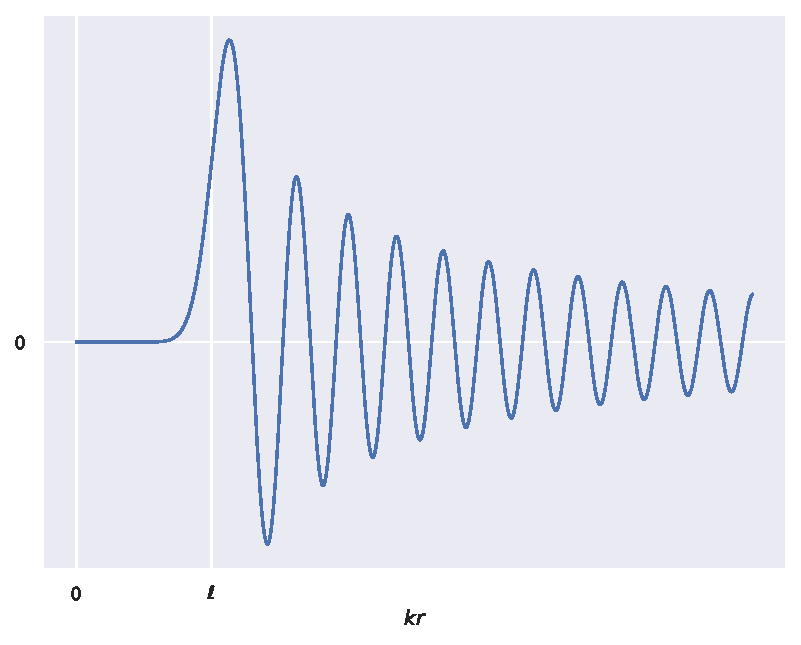
\includegraphics[width=\textwidth]{spherical_bessel.pdf}
	\caption[
		An example spherical Bessel function of the first kind
	]{
		An example spherical Bessel function of the first kind \(\bessel{k r}\) for some \(\ell{}\) highlighted on the plot.
		The Bessel functions peak sharply near \(k r = \ell{}\), and are \(\mathcal{O}{(k r)}^{\ell}\) for small \(k r\).
		Thus, the multipoles \(\ell{}\) predominately probe the spatial structure in three-dimensional fields with wavenumber \(k \almost{\ell/r}\).
		Projecting a plane wave over a sphere of radius much less than the wavelength cannot generate small-scale anisotropies --- reflected by the smallness of the Bessel functions at high \(\ell{}\) for small \(k r\).
		The Bessel functions tails are oscillatory which means that some power from a given \(k\) does also enter large-scale anisotropy.
		This arises from Fourier modes that are not aligned with their wavevector perpendicular to the line-of-sight.
	}\label{fig:chapter2_spherical_bessel}
\end{figure}
